\documentclass[12pt]{article} 
\usepackage[spanish]{babel}
\usepackage[utf8]{inputenc} 
\usepackage[left=1.50cm, right=1.50cm, top=1.50cm, bottom=1.50cm]{geometry}
\usepackage{blindtext}
\usepackage{multicol}
\usepackage{graphicx}
\usepackage{amsmath}
\usepackage{listings}
\usepackage{xcolor}

\title{Ecuación general de segundo grado en C}
\author{Gustavo Ramos}
\date{10 de Enero de 2024}

\definecolor{codegreen}{rgb}{0,0.6,0} 
\definecolor{codegray}{rgb}{0.5,0.5,0.5}
\definecolor{codepurple}{rgb}{0.58,0,0.82} \definecolor{backcolour}{rgb}{0.95,0.95,0.92} 
\lstdefinestyle{mystyle}
{ 
	backgroundcolor=\color{backcolour},
	commentstyle=\color{codegreen}, 
	keywordstyle=\color{magenta}, 
	numberstyle=\tiny\color{codegray}, 
	stringstyle=\color{codepurple}, 
	basicstyle=\ttfamily\footnotesize, 
	breakatwhitespace=true, 
	breaklines,
	captionpos=b,  
	keepspaces=true, 
	numbersep=5pt, 
	showspaces=false, 
	showstringspaces=false, 
	showtabs=false, 
	tabsize=2 
} 
\lstset{style=mystyle}

\begin{document}
	\maketitle
	\begin{abstract}
		Este documento expone un código que, de un archivo externo, lee datos pertenecientes a propiedades de los elementos de la tabla periódica y que, al decirle un numero, te devuelve el elemento perteneciente a esa posición.
	\end{abstract}
	\newpage
	\tableofcontents
	\newpage
	\begin{multicols}{2}
		\section{Introducción}
			La tabla periódica fue creada con el propósito de que las personas no tuvieran que aprenderse todos los elementos y sus características, pues si tomamos solo cinco características para los 118 elementos, serian en total ¡590 datos! (una barbaridad) y, irónicamente, las universidades hacen a sus alumnos de química aprenderse más de 700 datos... así que el propósito de la tabla periódica es... ser una referencia.
		\section{Antecedentes}
			La primera clasificación de los elementos químicos fue agruparlos en metales y no metales, atendiendo a sus características y propiedades.
			\subsection{Tablas de Döbereiner}
				Uno de los primeros pasos para la clasificación de los elementos se debe al químico alemán J. W, Döbereiner al establecer que había grupos de tres elementos (triadas), en los cuáles el elemento intermedio tenía una masa atómica de valor medio entre los otros dos elementos que formaban la triada. Son ejemplos de triadas: calcio estroncio bario; cloro bromo yodo; litio sodio potasio; azufre selenio teluro. Se llegaron a identificar hasta 20 triadas.
			\subsection{Octavas de Newlands}
				J. A. R. Newlands, profesor de Química en distintos centros de Londres, ordenó los elementos por orden creciente de masa atómica y observó que el octavo elemento, a partir de uno cualquiera, podía considerarse como una repetición del primero, de modo análogo a las notas de una escala musical. La primera octava estaba formada por los elementos: Li, Be, B, C, N, O, F. La segunda octava era: Na, Mg, Al, Si, P, S, Cl y son parecidas, respectivamente a las de la primera octava. Esta distribución coincide, en su mayor parte, con los periodos 2 y 3 de la tabla de Mendeléiev. El proceso de agrupamiento en ocho elementos no pudo extenderse más allá de las dos primeras octavas.
			\subsection{La tabla de Mendeléiev}
				Los intentos parciales de agrupación de los elementos químicos fueron superados por Dimitri Ivánovich Mendeléiev (1834-1907), quien ordenó los 63 elementos entonces conocidos por orden creciente de masa atómica y los vació en su tabla periódica. En ella los periodos
				(filas) tienen distintas longitudes y no se limitan a ocho elementos como decía Newlands. En las columnas (grupos) quedaban elementos con propiedades características parecidas y comportamientos químicos equivalentes. Ese fue su gran triunfo.
		\section{Metodología}
			\subsection{La tabla Periódica}
				En la tabla periódica actual los elementos están ordenados por orden creciente de número atómico. El número atómico es el número de protones que tiene un átomo en su núcleo. Coincide con el número de electrones en los átomos neutros, pero no así en los iones. Los iones positivos tienen menos electrones que protones y los negativos más electrones que protones.
	\end{multicols}
				\begin{center}
					\includegraphics[scale=0.9]{tabla.jpg}
				\end{center}
	\begin{multicols}{2}
				Como vemos en la imagen, los elementos parecen organizarse de manera simétrica (siendo el único que parece no encajar el Hidrógeno), se acomodan por tipo, masa, grupo y numero atómico.
		\section{Análisis y resultados}
			\subsection{Estructuras de datos en c}
				Para consultar los datos desde un archivo externo, se recurre a un \textbf{struct}, el cual es una declaración de tipo de datos compuestos que define una lista de variables agrupadas físicamente bajo un nombre en un bloque de memoria, lo que permite acceder a las diferentes variables a través de un solo puntero.\\
				El tipo de datos \textbf{struct} puede contener otros tipos de datos, por lo que se utiliza para registros de tipos de datos mixtos, como una entrada de directorio del disco duro (longitud del archivo, nombre, extensión, dirección física, etc.), u otros registros de tipo mixto (nombre , dirección, teléfono, saldo, etc.).\\
				\subsubsection{Declaración}
					 \lstinputlisting[language=c]{Estructura.c}
			\subsection{Resultados}
				Al programa le podemos pedir un elemento químico basándonos en su numero atómico, por ejemplo, el elemento $1$
				\begin{center}
					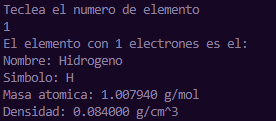
\includegraphics[scale=0.9]{1.png}
				\end{center}
				Para el elemento $105$
				\begin{center}
					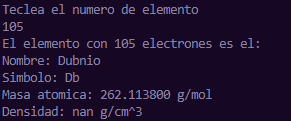
\includegraphics[scale=0.9]{2.png}
				\end{center}
				Y para los elementos $114$ y $65$
				\begin{center}
					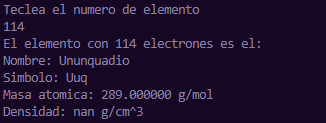
\includegraphics[scale=0.9]{3.png}
				\end{center}
				\begin{center}
					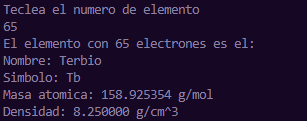
\includegraphics[scale=0.9]{4.png}
				\end{center}
		\section{Conclusiones}
			Las estructuras (\textbf{struct}) ayudan a acceder a los datos de manera más sencilla y compacta, aunque en un inicio el programa dio varios problemas ya que no reconocía los datos, sin embargo, al encontrar el problema (el orden), la lectura fue muy sencilla y ágil.
	\end{multicols}
	\appendix 
	\section{Diseño del código} 
		\lstinputlisting[language=c]{../main.c}
	\begin{multicols}{2} 
		\section{Referencias} 
			$[1]$ Casalderrey, M. L. (2019). En el año de la tabla periódica. Mol: boletín de la Sociedad de Ciencias de Galicia.\\
			$[2]$ Kelley, Al; Pohl, Ira (2004). A Book On C: Programming in C (Fourth ed.). pp. 418. ISBN 0-201-18399-4.\\
	\end{multicols} 
\end{document}